\documentclass[../main.tex]{subfiles} 

\renewcommand{\imageSrc}{../images/}
\renewcommand{\codeSrc}{../code/}


\begin{document}
\chapter{ASG Language}
ASG is a graphical specification language for distributed real-time systems and belongs to the family of hierarchical state languages such as \textit{STATECHARTS}, \textit{TTM} (Timed Transition Models) and \textit{MODECHARTS}. All these languages have been introduced progressively from 1987. The allow to describe the behavior of systems and have enhanced the expressiveness of state machines by introduction of time, hierarchies and parallelism. This avoids the explosion of the number of states and allows reasoning at different abstraction levels. It was intended to be readable by non computer-scientists, in order to be able to verify that what is specified is actually what the "client" wants.
\\\\
ASG, which was developed by UCLouvain, has some specific characteristics. 
\begin{itemize}
	\item It takes into account the impossibility to detect instantaneously a state change in a distributed system if it happens in a remote location (transmission delay) comment.
	\item It offers more restrictive rules on the destination state of a transition, e.g. it is not allowed to go to any other state that the initial sub-state of a state refined in sub-states if not coming from another sub-state of the same refinement. This allows to reason at a given hierarchical level without considering what happens at lower levels  comment. Consequently this promotes a top-down design, by refining states into sub-states when appropriate.
\end{itemize}

\section{Language Elements}
An ASG diagram consists of \textbf{states} and \textbf{transitions}. Crossing a transition is instantaneous: the system is thus always in a state.
\begin{figure}[h!]
    \centering
    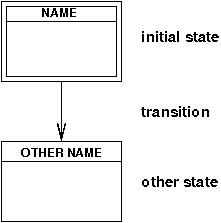
\includegraphics[width=0.25\textwidth]{\imageSrc/asg1.jpg}
    \caption{ASG States and Transitions}
    \label{asg1}
\end{figure}

\subsection{States}
Each state has a name and some \textbf{time-related state properties:}
\begin{itemize}
	\item \textbf{MINVT}: The \textbf{minimum visit time} is the minimum time the system remains in the state.
	\item \textbf{Time-Out}: A time-out counter is started when the state is entered. When this time-out elapses, a boolean variable \texttt{state\_name.timout} becomes true if the system is still in that state. 
\end{itemize}

A state has an \textbf{action} which is executed when the state is entered. When the action is finished, the system might choose to wait in the current state.  Executing the action takes some time and can be seen as happening in parallel with the system staying in the state. An action consists of 3 steps:
\begin{enumerate}
	\item Read the necessary data
	\item Process the data
	\item Write the results atomically
\end{enumerate}
An action has one property: its \textbf{deadline}, the maximum amount of time the action is allowed to take. The deadline is a declarative temporal specification: the system should be fast enough to respect that constraint. However, since the system assumes that deadlines are always respected, it's ignored by the system and a constraint for the implementer. On the other hand, \textbf{MINVT} and \textbf{time-outs} are elements that the system's behavior has to take into account.
\\\\
Further properties of a state include a \textbf{rendez-vous label}. This is used to synchronize parallel behavior. Another propertyi is a list of \textbf{resources} to prevent parallel behavior to reach incompatible states.

\subsection{Transitions}




\end{document}